\section{Sensory Aids}
In the last decade, drastic improvements in processing power and sensor technology have made visual and auditory assistive technologies (AT) more effective. A typical system for both visual and auditory ATs consists of a combination of a sensor as a substitute for the lacking sense and a feedback modality to inform the users in a way that they can process the information via their remaining functional senses. In this section, we will explore the most recent advancements in this field of ATs. 

\subsection{Visual Impairments}
\begin{figure}[h!]
    \centering
    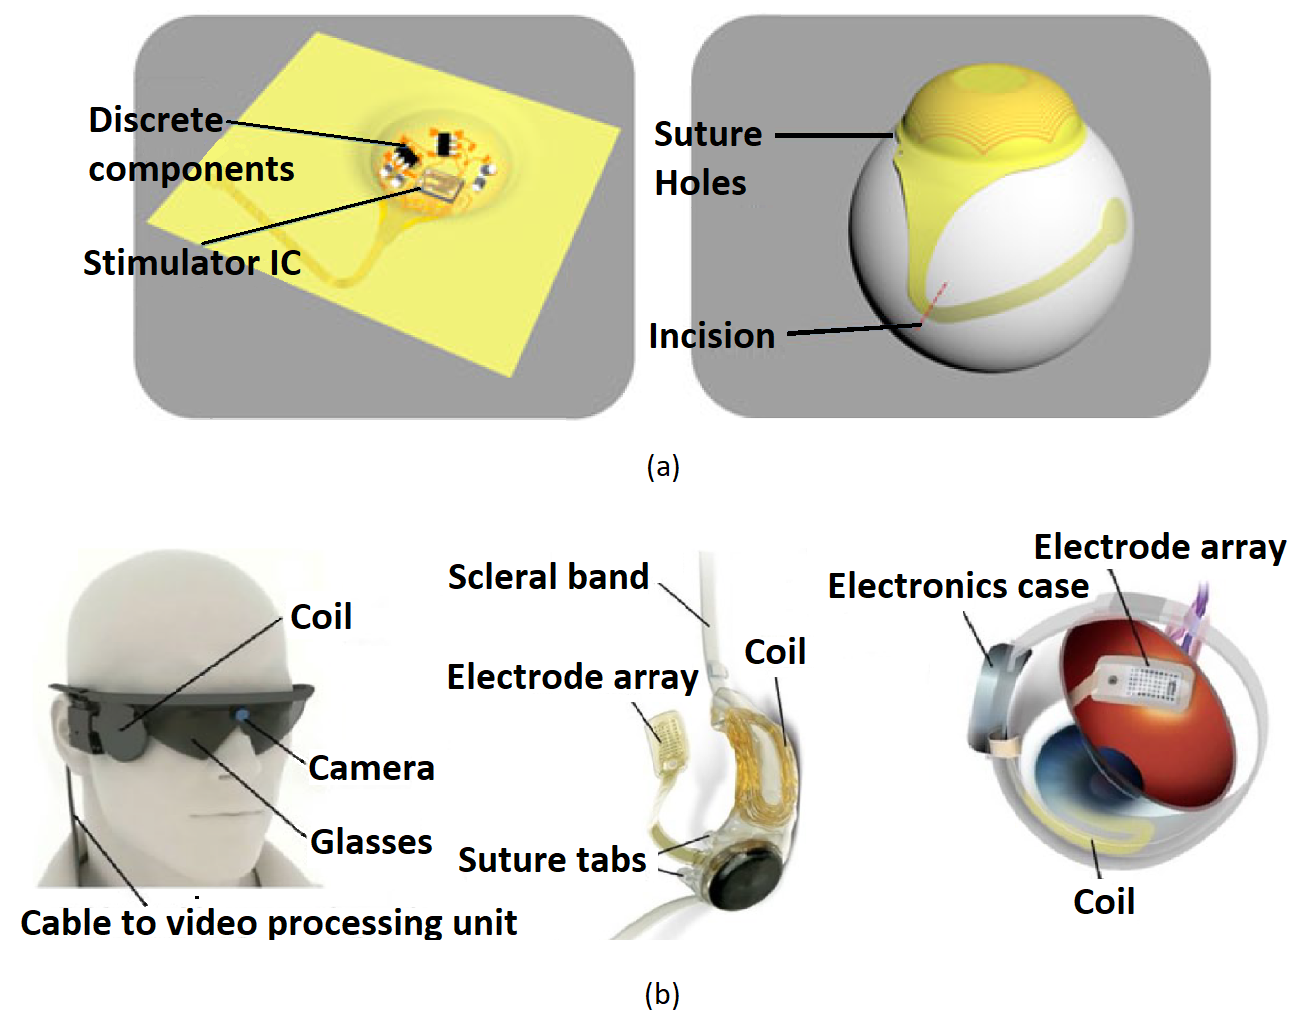
\includegraphics[width=110mm]{Figure/SensoryAid/VICollage}
    \caption{Schematic illustrations and photographs of visual impairment aids. (a) Illustration of LCP packaged monolithic retinal prosthesis system. (b) Illustration of Argus II epiretinal implant system.}
    \label{fig:VICollage}
\end{figure}

The level of visual impairment among individuals varies from moderate to profound and is classified by the Snellen visual acuity scale. In such a scale, the individual with impairment is asked to read individual letters placed a certain distance apart and are given a score compared to the healthy average. For example, 20/60 vision means that the visually impaired individual needs to be 20 feet away to see something that a healthy individual could see from 60 feet. More severe than visual impairment, legal blindness is defined as ``a visual acuity of 20/200 or a visual field of 20 degrees or less" according to the American Foundation for the Blind \parencite{AFB}. 

Visual aids are meant to help individuals suffering from any of the categories of blindness and low vision described above. These aids can be broadly divided into the categories of non-invasive and invasive devices. The former category of devices try to substitute vision with another sensing modality such as hearing. Therefore, range finding sensors such as ultrasonic sensors in conjunction with some form of sensory feedback are frequently used. In contrast, the invasive devices try to improve vision directly. For example, photodiode arrays are used in subretinal implants. 
 
There have been many ATs proposed in the literature recently in the sensory substitution category. One such paper, \textcite{kim_3-d_2020}, describes the use of ultrasonic sensors that are mounted on a glasses-like device to communicate object detection information in the user's field of view via sound. A total of three ultrasonic sensors are used, tilted at a 23$^{\circ}$ angle in the vertical direction with respect to each other to avoid interference. Object proximity to the user is communicated by both pitch and volume. The pitch describes if the object is in the top, center, or bottom of the sensors' field-of-view. The volume distinguishes how far the object is, with 10-step volume resolution. As an example, if the user is going towards the curb of a sidewalk, the sound produced by the device might be a 2-step, $C_3$ pitch sound. In contrast, if the user approaches a perpendicular tree branch at head height at the edge of the sensor's distance detection range, the device would emit a 10-step, $C_5$ pitch sound. 

In the invasive device market, retinal implants have shown efficacy as a long-term solution. \textcite{bloch_advances_2019} identifies three categories of retinal prosthetic devices: epiretinal, subretinal, and suprachoroidal and gives examples of commercial options for each. Epiretinal implants have found the most commercial success. The Argus II device \parencite{SecondSightMedical} consists of an external glasses-mounted camera and processing unit that records the environment as shown in Figure \ref{fig:VICollage}. The recorded image is then sent by modulating the RF power carrier to a coil and implant electronics implanted near the temple. From here the associated stimulus pulses are delivered via a flexible cable to the epiretinal stimulator electrode array that is surgically fixed to the surface of the retina. An advantage of this device is the well-developed surgical procedure. However, the drawbacks lie in the fact that stimulation of neurons behind the retina would require higher stimulation current levels and the device is susceptible to adverse events such as the degradation of the RF link due to misalignment of the coils, which can render the device instantly nonfunctional. Subretinal prostheses are unique because they use a photodiode array to generate photocurrent powered by light hitting the retina. This is in contrast to an epiretinal implant that uses an external camera. Though the photocurrent alone is not enough to elicit retinal stimulation, a simple external power unit can provide the necessary power for this device to be functional. Moreover, since electrodes are closer to the neurons behind the retina, lower levels of stimulation current are required.  

The Alphs IMS and AMS, designed by the company Retina Implant AG that has since gone out of business, are two devices that use the described subretinal implant mechanism. Finally, suprachoroidal prostheses have also been explored by some research groups. Leveraging the vast experience gained from cochlear implants, the Bionic Vision Australia group designed a 24-channel system that was implanted and tested \parencite{BionicVision}. The device showed some promise in terms of improvement in visual acuity; however, there were complications with the surgical procedure. Additionally, due to array distance from the retinal neurons the amount of stimulation current required was relatively high which poses some technical and safety challenges. 

Despite being available commercially since the 1980s \parencite{bloch_advances_2019}, there is still an ongoing research effort in the field of retinal implants targeting deficiencies in currently available devices. One of those deficiencies is the packaging used in epiretinal devices for the stimulator connected to the retina. Following the lead of packaging used in the established field, such as cochlear implants, retinal implants have traditionally used titanium-based encapsulation. The main benefits of this approach are that titanium is biocompatible, corrosion resistant, and has a high strength-to-density ratio. These properties make it a desirable packaging material for implants \parencite{jeong_miniaturized_2015}. Additionally, for cochlear implants that are generally fixed to a point inside a bone behind the ear, the device movement is not a major concern, while it is one of the major drawbacks of using such encapsulation for retinal implants. 

\textcite{jeong_miniaturized_2015} proposes a new polymer-based material for packaging with greater stiffness than a traditional MEMS device but less stiffness than the commercially-used titanium encapsulation. The argument made is that using biocompatible liquid crystal polymer will improve the user experience and the robustness of the solutions because it is conformable to the retinal surface as well as being sturdy enough to withstand the wear and tear associated with being implanted in the body. 

\subsection{Auditory Impairments}
\begin{figure}[h!]
    \centering
    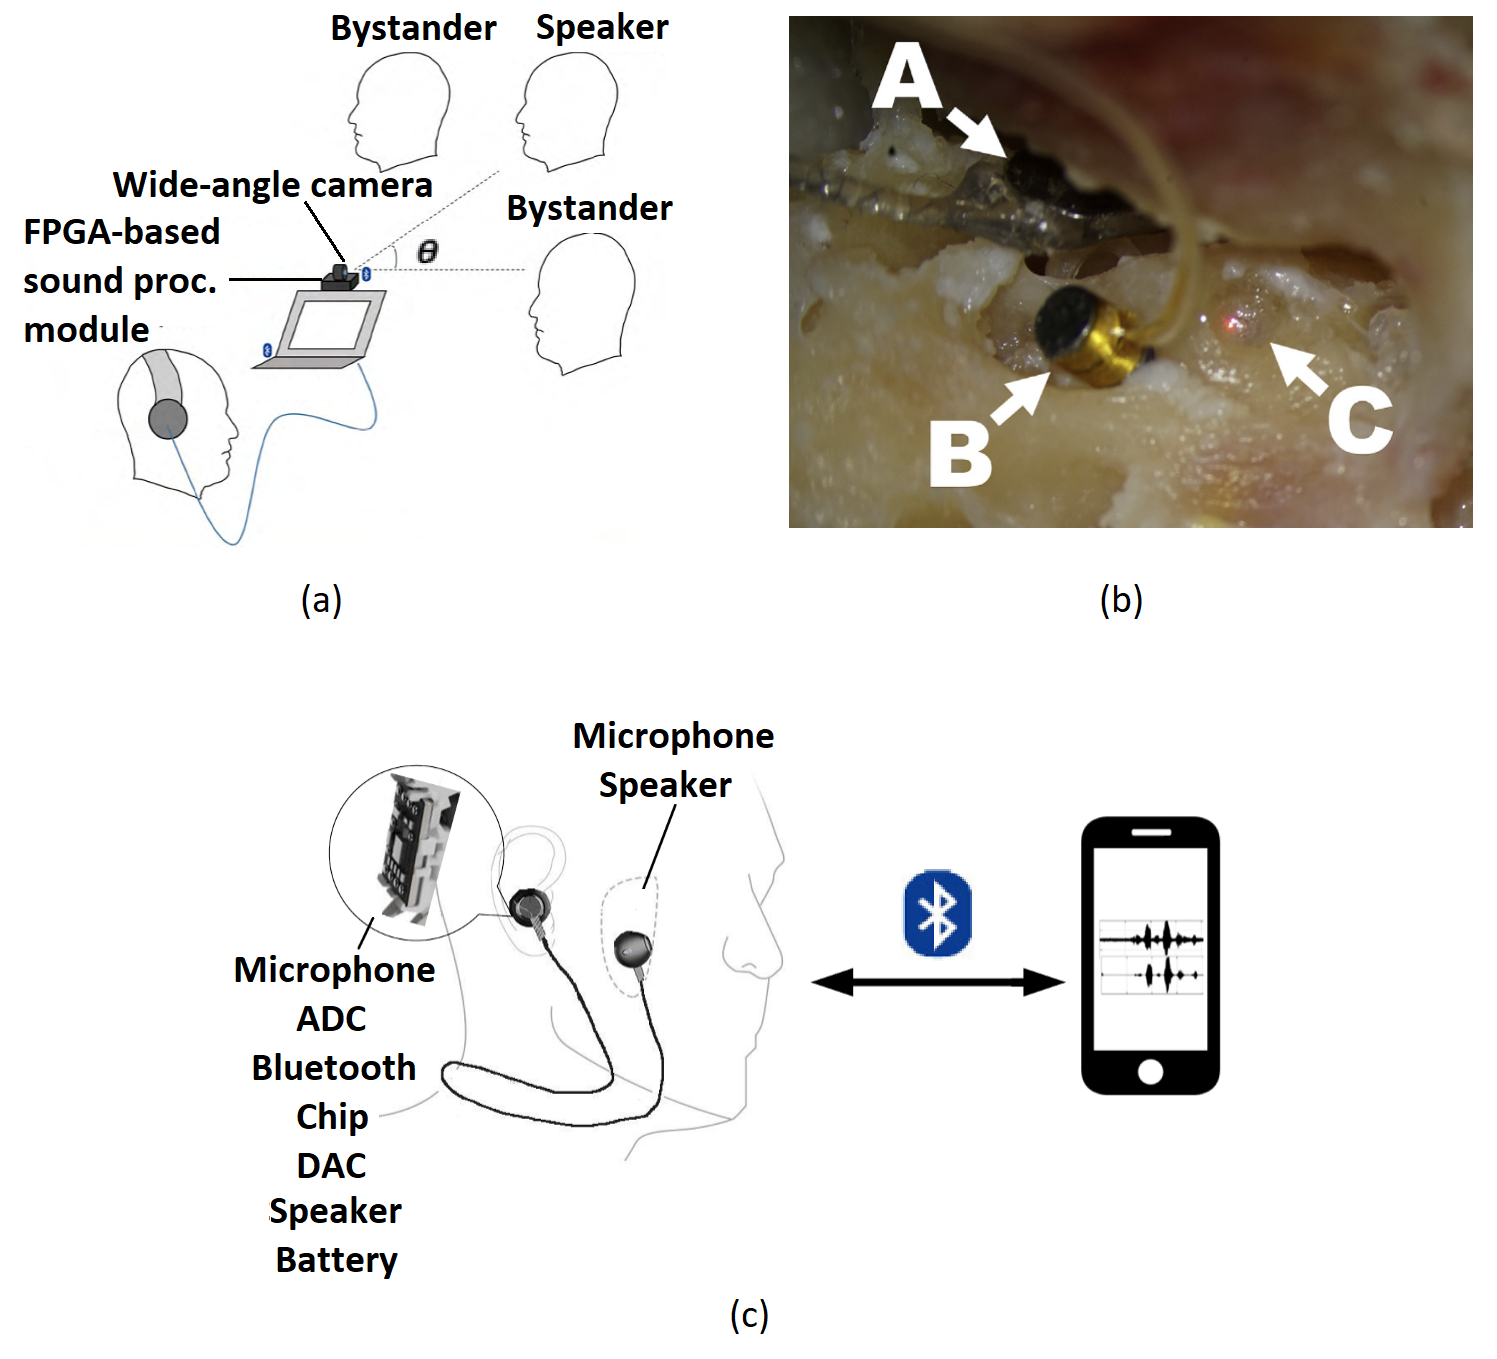
\includegraphics[width=100mm]{Figure/SensoryAid/AICollage}
    \caption{Schematic illustrations and photographs of auditory impairment aids. (a) Illustration of wide angle camera setup to locate and eliminate sources of noise based on spatial differentiation. (b) Photograph of piezoelectric sensor placed in incudostapedial joint as a way to eliminate the need for an external microphone. (c) Illustration of hearing aid system using deep learning algorithms processed on a generic smartphone.}
    \label{fig:SensAidCollage}
\end{figure}
\tab Auditory impairments, like visual impairments, can be classified by their severity. The classification is based on the tone loss. On the low end of the scale, the average tone loss for individuals with first degree moderate hearing loss is 41 dB to 55 dB. On the other extreme, individuals with cophosis (i.e. total hearing loss) have an average tone loss exceeding 120 dB \parencite{IBFA_audiometric_1996}. 

\tab The recent literature regarding auditory impairments suggests the potential solutions under two categories: invasive or non-invasive. In the latter category, external hearing aids are common. Research in this area mainly focuses on improving older designs by taking advantage of modern sensors and signal processing techniques. \textcite{lin_design_2019} tackles the issue of low signal strength in hearing aids by using cameras to locate the speaker and implement an adaptive beamforming method. Adaptive beamforming is a signal processing technique that improves the signal strength in a particular direction by combining sounds from an array of microphones with specific delays. As a result, the beamforming technique can separate noise and signal using spatial information, which is beneficial for improving hearing aid speech intelligibility. The authors propose the use of image processing and machine learning (ML) algorithms to detect where the speaker is and use this information to calculate the difference in time of arrival from different speakers. A field-programmable gate array (FPGA) is used to code the logic that will convert live video from a wide-angle camera into spatial information used in the adaptive beamforming technique. After testing, the proposed system improved the signal-to-noise ratio of sound from a noisy environment by ~5 dB. 

\textcite{li_smart_2020} also takes advantage of ML algorithms; the technique presented uses a smartphone rather than an FPGA to do the processing. The motivation behind this is to take advantage of the ubiquitous nature of smartphones. This proposed device implements a real-time deep learning (DL) algorithm to enhance recorded speech that is then played by the person's hearing aid. The microphone first picks up the sound, which is then transmitted via Bluetooth to the user's smartphone. The smartphone stores the signal in a buffer, which output is processed by the DL algorithm in real-time. With an average delay of 4-6 ms, the data is then transmitted back to the a speaker that plays the sound back to the user. Testing of the device showed that the DL algorithm improved the signal-to-noise ratio by a minimum of 20\%.

Pivoting now to invasive devices, receiving cochlear implants (CI) is a well-established and accepted treatment for hearing loss. As of 2011, over 220,000 individuals worldwide had received CIs according to \textcite{cosetti_cochlear_2011}. This paper reviews commercially available devices and compares them based on several technical features. The three most common commercial CIs including the HiRes devices \parencite{advanced_bionics}, Nucleus devices \parencite{cochlear_nucleus_systems}, and MAESTRO devices \parencite{med_el_2_maestro}. Mainly, the focus is on the most recent efforts of these companies to improve their respective devices to get better spatial specificity within the cochlea. A number of factors limit this specificity, including inner ear fluid that moves the stimulator, interference between adjacent electrode sites, and the distance between the stimulating electrode and the ganglia neurons. 

The HiRes CI series uses a Fidelity 120 \parencite{advanced_bionics_fidelity120} processing strategy that uses current steering to not only reduce adjacent electrode interference, but to also create "virtual" channels. Additionally, a preprocessing strategy implemented prior to the transmission to the implanted stimulator works to reduce noise immediately following recording by the microphone. As a result, the HiRes devices have shown better pitch and tone discrimination, directly related to improved speech perception. The Nucleus devices also use processing and preprocessing steps. The preprocessing step improves the audio source by using an adaptive directional microphone. Going further, a special modiolar-hugging electrode is used that helps physically space out the electrodes in the most optimized manner while maintaining closeness to the ganglia neurons. The processing step eliminates duplicate or masked sounds before stimulation. Finally, the MED-EL MAESTRO line of devices uses simultaneous stimulation of cochlea sections to improve speech perception versus the traditional sequential approach. Like the previous device, a custom FlexEAS electrode is used to appropriately space the electrodes while having the added benefit of maintaining existing inner ear functionality. Similar to the Nucleus devices, the MED-EL devices also use titanium packaging for stimulators rather than ceramic ones to reduce the size and increase usage in pediatric users.

Current research in the field of CIs explores ways to improve an established technology. \textcite{esinger_sensor-actuator_2019} looks at how to make a CI fully implanted by omitting the external microphone in exchange for a Floating Mass Transducer (FMT). The operating principle of the FMT is to record external sound by picking up vibrations in the long process of the incus. The vibrations are converted into a sound signal through the use of a piezoelectric sensor that is surgically placed in the incudostapedial joint. With this modification, the CI would be completely implanted in a single surgery, which could be beneficial for users who find it inconvenient to have a bulky external microphone placed on the side of their head. In this prospective device, an inductive link could be used to power the device. 

\subsection{Sensors in Use}
\tab In this section, we will explore some of the sensors unique to this area of sensory a devices in more detail.

\subsubsection{Photodiode Array}
A photodiode is essentially a PN junction where the P+ and N+ substrates are separated by a depletion region formed through the combination of holes and electrons. The size of the depletion region is affected by the magnitude of a reverse bias voltage applied to the diode. When light strikes the diode with a wavelength of less than 1100 nm \parencite{ida_sensors_2013} to exceed the bandgap energy of silicon, the electrons in the valence band are energized and move to the conduction band causing the current to flow. The amount of light striking the photodiode is therefore directly proportional to the amount of current generated. In \textcite{bloch_advances_2019}, subretinal implant devices are described that use photodiode arrays placed directly on the retina to generate photocurrent from light entering through the pupil.

\subsubsection{Piezoelectric Sensor}
The piezoelectric effect is a phenomenon where specific types of material (e.g. quartz, topaz etc.) produce an electric charge proportional to the mechanical stress applied to them \parencite{ida_sensors_2013}. Furthermore, the geometric strain of these materials is proportional to changes in the applied electric field. In \textcite{esinger_sensor-actuator_2019}, the authors use a sensor made of a piezoelectric material to remove the external component of the CI by converting the vibrations caused by sound in the long process of the incus into charge. By doing this, the piezoelectric sensor replaces the functionality of a microphone.

